% !TEX TS-program = pdflatexmk
\documentclass[12pt]{article}

% Layout.
\usepackage[top=1in, bottom=0.75in, left=1in, right=1in, headheight=1in, headsep=6pt]{geometry}

% Fonts.
\usepackage{mathptmx}
\usepackage[scaled=0.86]{helvet}
\renewcommand{\emph}[1]{\textsf{\textbf{#1}}}

% Misc packages.
\usepackage{amsmath,amssymb,latexsym}
\usepackage{graphicx}
\usepackage{array}
\usepackage{xcolor}
\usepackage{multicol}
\usepackage{tabularx,colortbl}
\usepackage{enumitem}
%to make tikz pics work
\usepackage{tikz,pgfplots}

\usepackage[colorlinks=true]{hyperref}

% Paragraph spacing
\parindent 0pt
\parskip 6pt plus 1pt
\def\tableindent{\hskip 0.5 in}
\def\ts{\hskip 1.5 em}

\usepackage{fancyhdr}
\pagestyle{fancy} 
\lhead{\large\sf\textbf{MATH F251: Calculus I}}
\rhead{\large\sf\textbf{Fall 2019}}
\chead{\large\sf\textbf{Quiz 1: SAMPLE B}}

\newcommand{\localhead}[1]{\par\smallskip\textbf{#1}\nobreak\\}%
\def\heading#1{\localhead{\large\emph{#1}}}
\def\subheading#1{\localhead{\emph{#1}}}

\newenvironment{clist}%
{\bgroup\parskip 0pt\begin{list}{$\bullet$}{\partopsep 4pt\topsep 0pt\itemsep -2pt}}%
{\end{list}\egroup}%

\usetikzlibrary{calc}
\pgfplotsset{my style/.append style={axis x line=middle, axis y line=
middle, xlabel={$x$}, ylabel={$y$}, axis equal }}

\begin{document}
\textbf{Directions:} The quiz contains 20 problems. Place your answer in the blank provided. For graphing questions, a set of axes are provided. All graphs must be labeled.
\begin{enumerate}
%%%%
%type: numerical simplification - exponential
\item Simplify ${\large{\left(\frac{8}{9}\right)^{-1/2}}}.$


\quad \hfill \underline{\hspace{2in}}
\vfill

%%%%
%type: equation of a line
\item Write the slope intercept form (that is, the form: $y=mx+b$) of the equation of the line containing the point $(2,3)$ parallel to the line $6x+2y=7.$


\quad \hfill \underline{\hspace{2in}}
\vfill

%%%%%%%%%%
%type: simplification with exponent rules
\item  Simplify the expression $\displaystyle{\frac{3x^2y-4x^3}{xy^2}}$. Write your answer without negative exponents.
%

\quad \hfill \underline{\hspace{2in}}
\vfill

%%%%%%%
%type: Questions from picture
\item Use the graph of $f(x)$ below to estimate $f(3).$
% 

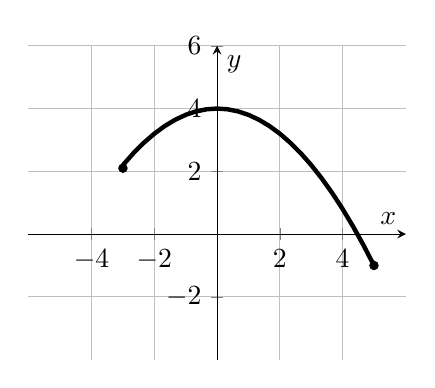
\begin{tikzpicture}
\begin{axis}[scale=.7, my style, xtick={-4,-2,...,4}, ytick={-2,2,4,6},
xmin=-4, xmax=4, ymin=-4, ymax=6,  
mark size=3.0pt, grid]
\addplot[domain=-3:5,ultra thick] {-0.2*((x)^2)+4};
\addplot[mark=*,mark size=1.5,only marks] coordinates {(-3,2.1)(5,-1)};
\end{axis}
\end{tikzpicture}
\quad \hfill \underline{\hspace{2in}}
\vfill

%%%%%%%
%type: expand and simplify
\item Simplify the rational expression: $\displaystyle{\frac{x+y}{1+\frac{1}{y}}}.$
%

\quad \hfill \underline{\hspace{2in}}
\vfill
\newpage

%%%%%%%
%type: solve an equation -- quadratic
\item Solve the equation $3x^2-2x-1=0.$
%

\quad \hfill \underline{\hspace{2in}}
\vfill

%%%%%%%
%type: piecewise defined function
\item Given the piecewise defined function below, determine the value(s) of $x$ such that $f(x)=3.$

$f(x)=\begin{cases} x^2 & x \leq 1 \\ x+3 & x >1 \end{cases}.$
\quad \hfill \underline{\hspace{2in}}
\vfill

%%%%%%%
%type: elementary numerical trig
\item Find the exact value of $\sin ( 2 \pi/3).$
%

\quad \hfill \underline{\hspace{2in}}
\vfill

%%%%%%%%%%
%type: misc
\item Find the equation for the top half of the circle with center $(0,0)$ and radius 3.
%

\quad \hfill \underline{\hspace{2in}}
\vfill

\vspace{1in}

%%%%%%%
%type: Difference quotient
\item For the function $f(x)=x^2$, find the expression $f(2)-f(2+h).$ Simplify your answer if possible.

\quad \hfill \underline{\hspace{2in}}
\vfill
\newpage
%%%%%%%%%%%%%
%type: inverse
\item Using the table of values for the function $f(x)$, determine $f^{-1}(2).$\\

\begin{tabular}{| c||c|c|c|c|c|c|c|c|c|c|}
\hline
$x$ &1&2&3&4&5&6&7&8&9&10 \\
\hline
$f(x)$&0.5&1&1.7&1.9&2&4&4.5&5.1&6.7&10.8\\
\hline
\end{tabular}
%

\quad \hfill \underline{\hspace{2in}}
\vfill
%%%%%%%%
%type: composition of functions
\item Let $g(x)=2x+1$, find $(g \circ g)(x).$ You do not need to simplify your answer.
% and 

\quad \hfill \underline{\hspace{2in}}
\vfill
%%%%%%%
%Solutions to equations
%%%%%%

%%%%%%%%%
%type: exponential or log
\item Solve for $x$ in the equation $\ln ( x^2-5)=4.$
%$\ln ( x^2-5)=4$

\quad \hfill \underline{\hspace{2in}}
\vfill

%%%%%%
%Domain problems
%%%%%%%%
%type: domain roots
\item Determine the domain of $f(x)=\frac{1}{1-\sqrt[3]{x}}.$ Give your answer in interval notation
%%

\quad \hfill \underline{\hspace{2in}}
\vfill

%%%%%%%
%type: trig function
\item Solve the equation $0=\tan x.$
%


\quad \hfill \underline{\hspace{2in}}
\vfill

%%%%%%%
%type: exponential or log
\item Find the exact value of the expression $\log_{10}(25)+\log_{10}(4).$
%


\quad \hfill \underline{\hspace{2in}}
\vfill

\newpage
%%%%%%%%%
%Sketching Problems
%%%%%%%%%
%type: graph 1/x
\item On the axes below, sketch the graph of $y=-\sqrt{x}.$
%

\begin{tikzpicture}[scale=0.6][>=latex]
%x axis
\draw[->] (-5 ,0) -- (5 ,0) node[below] {$x$};
\foreach \x in {-4,...,4}
\draw[shift={(\x,0)}] (0pt,2pt) -- (0pt,-2pt);
%y axis
\draw[->] (0,-5) -- (0,5) node[left] {$y$};
\foreach \y in {-4,...,4}
\draw[shift={(0,\y)}] (2pt,0pt) -- (-2pt,0pt);
%\node[below left] at (0,0) {\footnotesize $0$};
\end{tikzpicture}
 \vfill

%%%%%%%
%type
\item On the axes below, sketch the graph of $y=2\sin(x)+3$ on the interval $[-2\pi,2\pi].$
%

\begin{tikzpicture}[scale=0.6][>=latex]
%x axis
\draw[->] (-5 ,0) -- (5 ,0) node[below] {$x$};
\foreach \x in {-4,...,4}
\draw[shift={(\x,0)}] (0pt,2pt) -- (0pt,-2pt);
%y axis
\draw[->] (0,-5) -- (0,5) node[left] {$y$};
\foreach \y in {-4,...,4}
\draw[shift={(0,\y)}] (2pt,0pt) -- (-2pt,0pt);
%\node[below left] at (0,0) {\footnotesize $0$};
\end{tikzpicture}
 \vfill


\vfill
%%%%%%%%%%%
%type: exponential or logarithm
\item On the axes below, sketch the graph of $y=\ln(x-1).$
%

\begin{tikzpicture}[scale=0.6][>=latex]
%x axis
\draw[->] (-5 ,0) -- (5 ,0) node[below] {$x$};
\foreach \x in {-4,...,4}
\draw[shift={(\x,0)}] (0pt,2pt) -- (0pt,-2pt);
%y axis
\draw[->] (0,-5) -- (0,5) node[left] {$y$};
\foreach \y in {-4,...,4}
\draw[shift={(0,\y)}] (2pt,0pt) -- (-2pt,0pt);
%\node[below left] at (0,0) {\footnotesize $0$};
\end{tikzpicture}
 \vfill

\item Solve the inequality $x^2-4 \geq 0.$

\quad \hfill \underline{\hspace{2in}}
\vfill

\end{enumerate}
\end{document}
